\item
\begin{enumerate}
  \item Implement the above Bayes net with the specified conditional probabilities into pgmpy. {\bf [2.5 points]}
        \begin{center}
          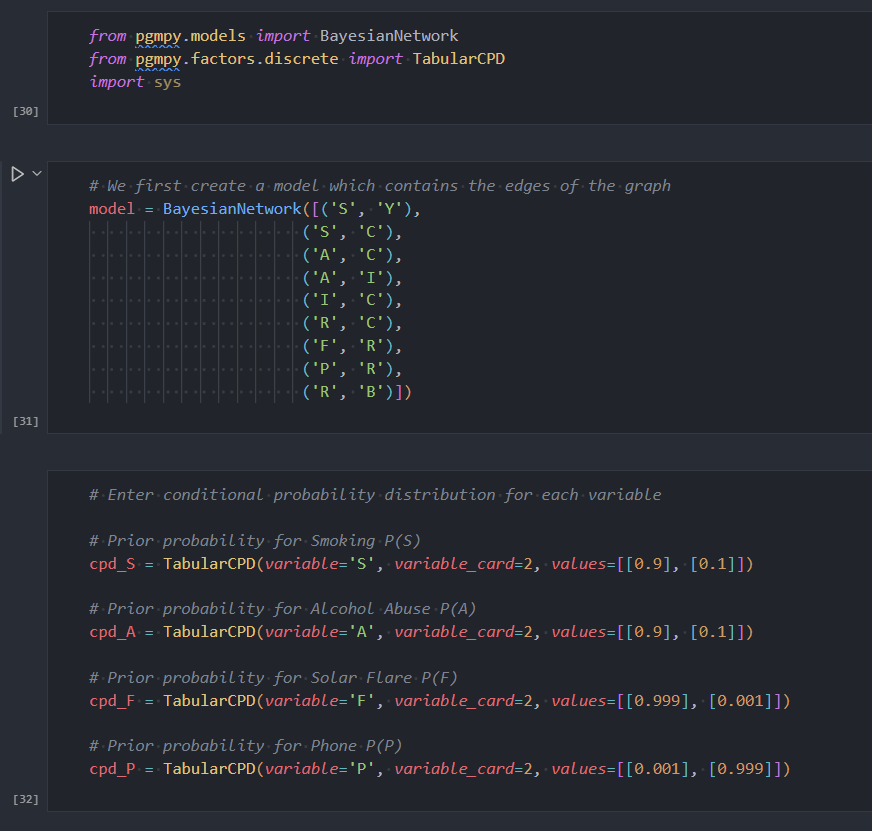
\includegraphics[scale=0.5]{"./Diagrams/Q3 Code Page 1.PNG"}
          
\includegraphics[scale=0.5]{"./Diagrams/Q3 Code Page 2.PNG"}
        \end{center}
        \clearpage
  \item Draw the Bayesian network clearly showing the nodes and arrows showing relationship among all the variables. {\bf [1.5 points]}
        \begin{center}
          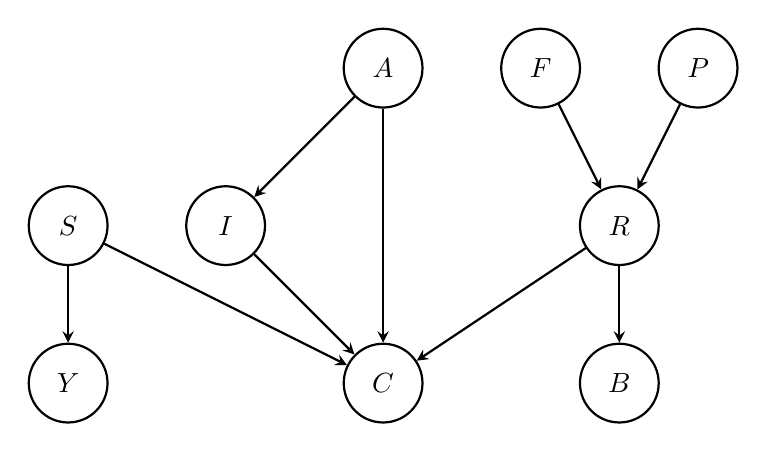
\begin{tikzpicture}[->,>=stealth,auto,node distance=0cm,
              thick,main node/.style={circle,draw}, minimum size=1cm]

            \node[main node] (S) at (0,2) {$S$};
            \node[main node] (Y) at (0,0) {$Y$};
            \node[main node] (I) at (2,2) {$I$};
            \node[main node] (A) at (4,4) {$A$};
            \node[main node] (C) at (4,0) {$C$};
            \node[main node] (F) at (6,4) {$F$};
            \node[main node] (R) at (7,2) {$R$};
            \node[main node] (B) at (7,0) {$B$};
            \node[main node] (P) at (8,4) {$P$};

            \path[every node/.style={}]
            (S) edge (Y)
            (S) edge (C)
            (A) edge (I)
            (A) edge (C)
            (I) edge (C)
            (F) edge (R)
            (P) edge (R)
            (R) edge (C)
            (R) edge (B);
          \end{tikzpicture}
        \end{center}
  \item What is the probability of radiation given cancer? Show values for $R\in\{0, 1\}$. {\bf [1.5 points]}
        $$P(R=1\mid C=1)$$
        \begin{lstlisting}
          from pgmpy.inference import VariableElimination
          infer = VariableElimination(model)

          # Get probability of Radiation given Cancer P(R=1 | C=1)
          phi_query = infer.query(['R'], evidence={'C':1}, joint = False)
          factor = phi_query['R']
          print('Probability of Radiation given Cancer')
          print(factor)

          # Output
          '''
          Probability of Radiation given Cancer
          +------+----------+
          | R    |   phi(R) |
          +======+==========+
          | R(0) |   0.9214 |
          +------+----------+
          | R(1) |   0.0786 |
          +------+----------+
          '''
        \end{lstlisting}
        \begin{align*}
          P(R=0\mid C=1) & =0.9214 \\
          P(R=1\mid C=1) & =0.0786
        \end{align*}
  \item What is the probability of cancer given the patient has skin burn, yellow fingers and abuses alcohol? Show values for $C\in\{0, 1\}$. {\bf [1.5 points]}
        $$P(C=1\mid B=1, Y=1, A=1)$$
        \begin{lstlisting}
          # Get probability of Cancer given skin burn, yellow fingers and alcohol abuse. P(C=1 | B=1, Y=1, A=1)
          phi_query = infer.query(['C'], evidence={'B':1, 'Y':1, 'A':1}, joint = False)
          factor = phi_query['C']
          print('Probability of Cancer given skin burn, yellow fingers and alcohol abuse')
          print(factor)

          # Output
          '''
          Probability of Cancer given skin burn, yellow fingers and alcohol abuse
          +------+----------+
          | C    |   phi(C) |
          +======+==========+
          | C(0) |   0.4296 |
          +------+----------+
          | C(1) |   0.5704 |
          +------+----------+
          '''
        \end{lstlisting}
        \begin{align*}
          P(C=0\mid B=1, Y=1, A=1) & =0.4296 \\
          P(C=1\mid B=1, Y=1, A=1) & =0.5704
        \end{align*}
  \item Are Smoking and skin burn independent given that cancer is present? Justify your answer. {\bf [1.5 points]}\\
        No. They are dependent.There is a V-structure between $S$, $C$ and $R$.
        $$S\rightarrow C\leftarrow R$$
        Given $C$, it couples $S$ and $R$. This makes $S$ and $R$ dependent. Since $R$ and $B$ are dependent due to cascade structure
        $$R \rightarrow B$$
        then $S$ and $B$ are dependent.
  \item What is the probability of cancer if you never abused alcohol or used a cellphone? {\bf [1.5 points]}
        $$P(C=1\mid A=0, P=0)$$
        \begin{lstlisting}
          # Get probability of Cancer given no alcohol and no cellphone. P(C=1 | A=0, P=0)
          phi_query = infer.query(['C'], evidence={'A':0, 'P':0}, joint = False)
          factor = phi_query['C']
          print('Probability of Cancer given no alcohol and no cellphone')
          print(factor)

          # Output
          '''
          Probability of Cancer given no alcohol and no cellphone
          +------+----------+
          | C    |   phi(C) |
          +======+==========+
          | C(0) |   0.8495 |
          +------+----------+
          | C(1) |   0.1505 |
          +------+----------+
          '''
        \end{lstlisting}
        \begin{align*}
          P(C=0\mid A=0, P=0) & =0.8495 \\
          P(C=1\mid A=0, P=0) & =0.1505
        \end{align*}
\end{enumerate}